\documentclass[a4]{article}

\usepackage{geometry}
\usepackage{graphicx}

\title{Supplementary figures for the article: "Quantitative characterisation of iridescent colours in biological studies: a novel method using optical theory"}

\author{Hugo Gruson, Christine Andraud, Willy Daney de Marcillac, Serge Berthier,\\ Marianne Elias, Doris Gomez}

\date{}

\begin{document}

    \maketitle
    
    \section*{Schematic representation of the goniometer used in this study}
    
    \begin{figure}[!h]
        \centering
        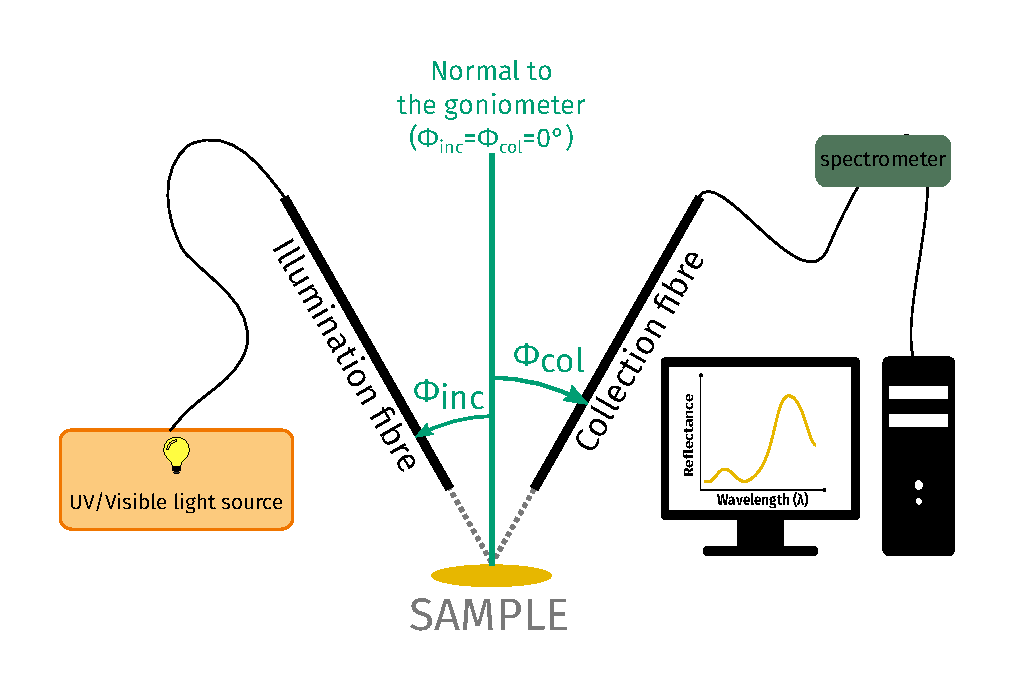
\includegraphics[width=0.6\textwidth]{gonio.pdf}
        \caption{Schematic representation of a goniometer with the illumination and collection fibres and their angle with the normal to the sample $\Phi_{inc}$ and $\Phi_{col}$. The sign of $\Phi_{inc}$ and $\Phi_{col}$ is figured by an arrow pointing towards the positive rotation direction.}
    \end{figure}
    
    \clearpage
    
    \section*{Range of parameters estimated for hummingbirds and butterflies}
    
    \begin{figure}[!h]
        \centering
        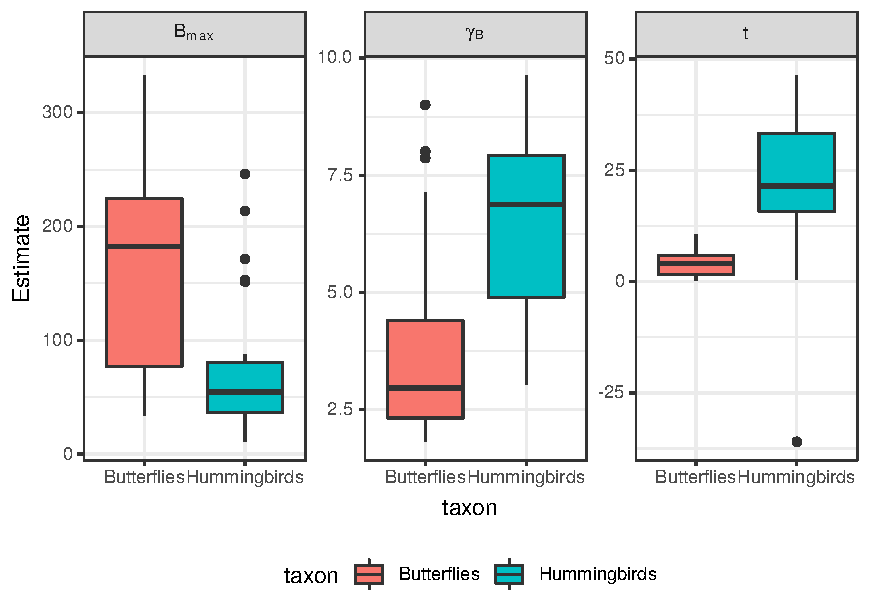
\includegraphics[width=0.7\textwidth]{boxplot_brightall}
        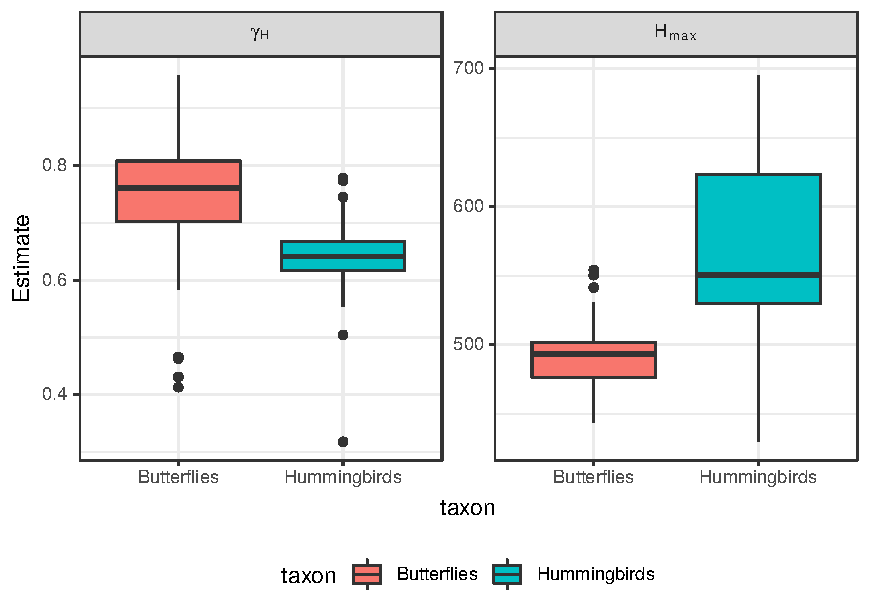
\includegraphics[width=0.7\textwidth]{boxplot_hueall}
        \caption{Both hummingbirds and butterflies display a large diversity of hues and brightness, as well as angle dependency in hue and brightness. The butterflies species we measured tend to have multilayer structure parallel to the sample surface (no tilt), which is not the case for hummingbird. The outlier for tilt in hummingbirds is the back of \textit{Aglaeactis cupripennis}.}
    \end{figure}
    
    \clearpage
    
    \section*{Tests for correlation between iridescence parameters}
    
    \begin{figure}[!h]
        \centering
        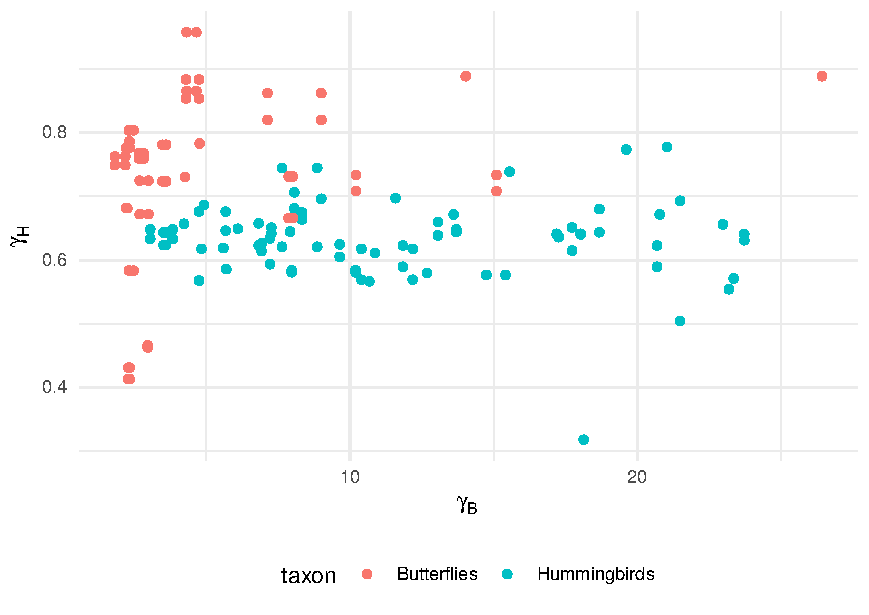
\includegraphics[width=0.75\textwidth]{cor_gammaB_gammaH}
        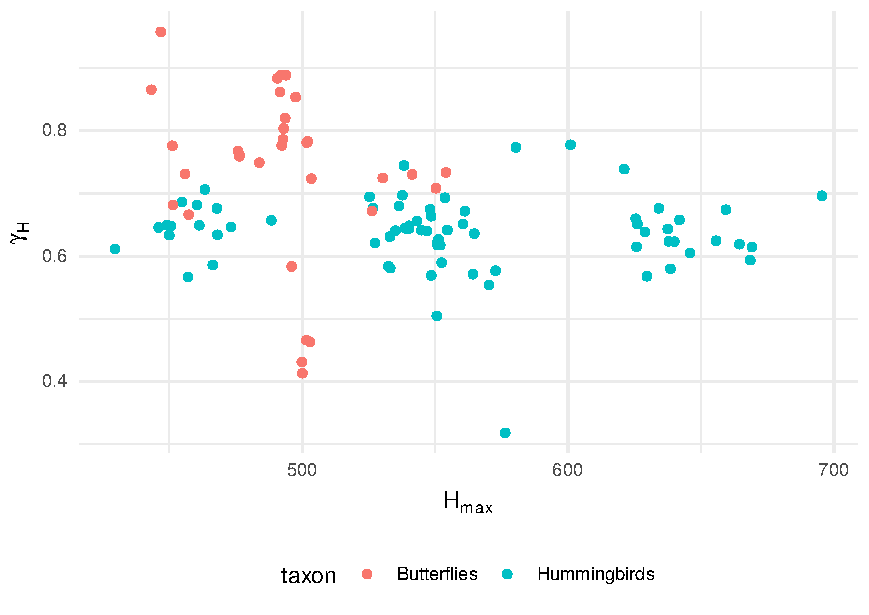
\includegraphics[width=0.75\textwidth]{cor_Hmax_gammaH}
        \caption{No correlation between hue and brightness angular dependency ($\gamma_{H}$ and $\gamma_{B}$ respectively) or between hue dependency and hue at a given angle ($\gamma_{H}$ and $H_{max}$).}
    \end{figure}
    
\end{document}